
\section{Expérimentation}
\label{editor:sec:experimentation}

\paragraph{Objectif :} Montrer que l'éditeur collaboratif décentralisé \CRATE
passe à l'échelle en termes de nombre d'utilisateurs et de taille de
documents.

\paragraph{Description :} Cette expérimentation construit des réseaux de 101 à
601 participants. Pour cela, des machines sont réservées sur le banc d'essai
Grid'5000. Sur chacune d'elles sont lancés un à plusieurs navigateurs Web
observant le processus d'intégration au réseau. Par exemple, 100 machines avec 6
navigateurs chacune permettent de créer le réseau à 601 participants -- le
participant supplémentaire étant le créateur du document hébergeant aussi le
serveur de signalisation.  Chaque session d'édition est en charge d'écrire un
document artificiel de plusieurs millions de caractères en insérant ceux-ci à la
fin du document. Les mesures concernent le trafic sortant moyen de chacun des
membres. Globalement, 100 opérations sont effectuées par seconde, uniformément
réparties entre les participants. La session dure 7 heures.

\begin{figure}
  \begin{center}
    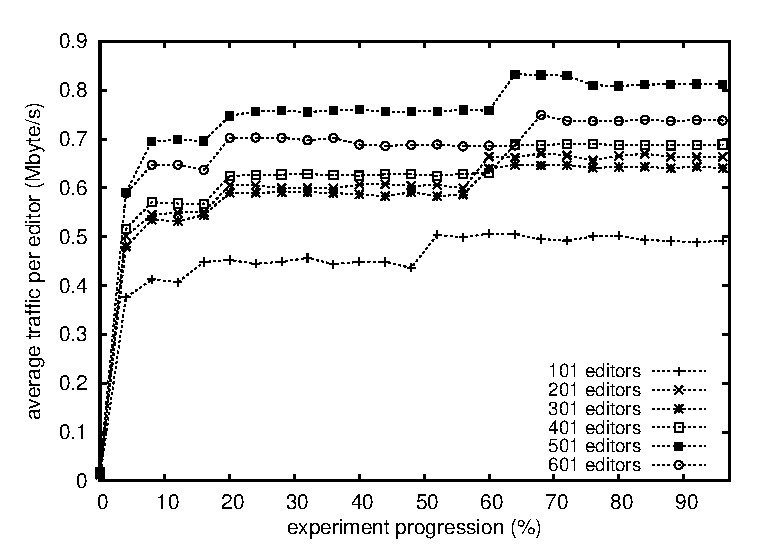
\includegraphics[width=0.8\textwidth]{img/editor/communication.eps}
    \caption[Trafic généré par \CRATE lors de sessions d'édition]
    {\label{editor:img:communication} Trafic moyen par seconde généré par chaque
      éditeur pendant la session d'édition. L'axe des abscisses montre la
      progression de l'expérimentation. L'axe des ordonnées montre le trafic
      moyen sortant par éditeur en mégaoctets par seconde.}
  \end{center}
\end{figure}

\paragraph{Résultat :} La figure~\ref{editor:img:communication} montre le
résultat de cette expérimentation.
\begin{inparaenum}[(i)]
\item Le trafic généré croît de façon polylogarithmique par rapport à la taille
  du document : plus l'expérience progresse, plus le nombre d'insertions
  effectuées dans le document est important, plus la croissance des identifiants
  diminue.
\item À cela s'ajoute un facteur multiplicatif logarithmique par rapport au
  nombre de participants : plus la session d'édition comporte de membres, plus
  le trafic généré est important. Toutefois, l'écart entre les mesures diminue
  tandis que le nombre de participants est incrémenté linéairement. On note
  toutefois des exceptions à ces observations. Par exemple, les mesures sur 501
  éditeurs dominent les mesures sur 601 éditeurs.
\end{inparaenum}

\paragraph{Explication :} \CRATE utilise \LSEQ
(cf. chapitre~\ref{repl:chap:lseq}). Le comportement d'édition des participants
est monotone. \LSEQ possède une complexité polylogarithmique sur ses
identifiants par rapport au nombre d'insertions effectuées dans la
séquence. Ainsi, plus les expérimentations progressent, plus le nombre
d'insertions dans la séquence augmente. Les messages envoyés ne comportant que
les identifiants de \LSEQ, la croissance du trafic hérite de cette croissance
polylogarithmique. \CRATE utilise \SPRAY (cf. §\ref{net:chap:spray}). Lorsqu'un
nouveau membre rejoint une session d'édition, il ajoute avec lui un nombre
logarithmique de connexions par rapport à la taille du réseau. Chacune de ces
connexions est activement utilisée par le mécanisme de diffusion de messages
afin que chacun des identifiants parvienne à tous les éditeurs. Pour chaque
opération locale effectuée, chaque membre retransmet le message à ses voisins
exactement une fois. Ainsi, chaque opération est transmise par chaque nœud à
leur vue dont la taille est logarithmique par rapport à la taille de la session
d'édition. Ainsi, une session d'édition à 100 participants génère moins de
trafic qu'une session d'édition à 200 participants. L'exception perçue entre
certaines configurations de l'expérimentation est due à l'aspect aléatoire du
processus d'entrée dans le réseau de \SPRAY. En effet, le nombre d'arcs ajoutés
dans le réseau dépend du nœud contact du nouvel arrivant. Si ce contact possède
plus de voisins que le logarithme recherché, alors la taille moyenne des vues
partielles augmentera d'autant plus; et inversement.  Sur un grand nombre
d'exécutions, l'effet aléatoire induit par les choix de contacts serait gommé.



%%% Local Variables:
%%% mode: latex
%%% TeX-master: "../../paper"
%%% End:
